\chapter{Abstract Dutch}
Tegenwoordig gebruiken moderne controlesystemen "model predictive control" algoritmes. Wanneer lineaire modellen worden gebruikt, moet een stelsel van lineaire vergelijkingen worden opgelost. De algoritmes voor het oplossen van een stelsel van lineaire vergelijkingen zijn uitgebreid onderzocht en geimplementeerd. 

Wanneer niet lineaire modellen worden gebruikt, moet een niet lineaire stelsel opgelost worden. Dit wordt typisch opgelost met een iteratief algoritme zoals "interior point" algoritmes. Deze algoritmes gebruiken veel geheugen wat ze vaak ondergeschikt maakt voor embedded toepassingen. Dit is waar het PANOC algoritme interessant wordt, het kan namelijk een niet lineaire stelsel oplossen met veel minder geheugen dan een "interior point" algoritme. Maar heeft aslook super lineaire convergentie.

Het doel van deze thesis is om een raamwerk te implementeren dat een niet lineaire MPC controller genereerd in C, die gebruikt maakt van het PANOC algoritme. De code is specifiek gericht aan embedded toestellen, waardoor PANOC een uitstekende keuze is. 


\chapter{Mathematical definitions}
	\section{Box function}
	\label{appendix:box function}
		1 dimension:
		\begin{equation}
			\boxfunction_{1D}(u) =
			\begin{cases}
				 1 & u \in [-U_b:U_b]\\
				 0 & \other
			\end{cases}
			\label{eq:box function 1 dimension}
		\end{equation}
		N dimensions:
		\begin{equation}
			\boxfunction(u) = \min\left[ \sum_{k=1}^ N \boxfunction_{1D}(u) \right]
			\label{eq:box function N dimensions}
		\end{equation}
	\section{Indicator Box function}
	\label{appendix:indicator box function}
		\begin{equation}
			I_{\boxfunction}(u)=
			\begin{cases}
				0 & u \in [-U_b:U_b]\\
				\inf & \other
			\end{cases}
		\end{equation}
		
		\begin{equation}
			\prox_{\gamma I_{\boxfunction}}(u)=
			\begin{cases}
				u & u \in [-U_b:U_b]\\
				-U_b & u \in [-\inf:-U_b)\\
				-U_b & u \in (U_b:\inf]\\
			\end{cases}
		\end{equation}
	\section{Conjugate of strongly convex function}
		\begin{equation}
			f^*(x)= \underset{u \in dom(f)}{<y,x>-f(y)}
		\end{equation}
		
		If $\nabla f^*$ is Lipschitz and obeys \eqref{eq:appendix f lip}, then $f^*$ is well defined and differentiable. (assume dom(f) is convex and closed)
		\begin{equation}
			\nabla f^*(x) = y^* = \argmax <y,x> - f(y)
		\end{equation}
		
		\begin{equation}
			|| \nabla f^*(x) - \nabla f^*(y) ||_2 \leq \mu^{-1} ||x-y||_2
			\label{eq:appendix f lip}
		\end{equation}
		
\chapter{Proof FBE alternate equation}

\begin{proof}
	$\varphi_{\gamma} =   f(x) + \underset{y}{\inf} \Big\{ \nabla f(x)^T(y-x) + g(y) + \frac{1}{2 \gamma} ||x-y||^2  \Big\} $
	\begin{align*}
	g^{\gamma} 	&=  \underset{y}{\inf} \big \{f(y)+\frac{1}{2 \cdot \gamma}||x-y||^2 \big \} \\
	\varphi_{\gamma} 
	&= f(x) - \frac{\gamma}{2}||\nabla f(x)||^2 + g^{\gamma} \big(x-\gamma \nabla f(x) \big) \\
	&= f(x) - \frac{\gamma}{2}||\nabla f(x)||^2 + g^{\gamma} \big(\bar{x} \big)\\
	g^{\gamma} (\bar{x})
	&=\underset{y}{\inf} \Big\{g(y)+\frac{1}{2 \gamma}||\bar{x}-y||^2 \Big\}	\\
	\bar{x}^T\bar{x}
	&=[x- \gamma \nabla f(x)]^T[x- \gamma \nabla f(x)] \\
	&= x^Tx -2x^T\nabla f(x) \gamma + \gamma^2 \nabla f(x)^T\nabla f(x)-2x^Ty \\
	&=-2(x-\gamma f\nabla(x))^Ty\\
	&=-2x^Ty + 2\gamma \nabla f(x)^Ty \\
	\frac{1}{2 \gamma}||\bar{x}-y||^2
	&=\frac{1}{2 \gamma} \Big [ (\bar{x}-y)^T(\bar{x}-y) \Big]\\
	&=\frac{1}{2 \gamma} \Big [ x^Tx - 2 x^Ty + y^Ty \Big]\\
	& =\frac{1}{2 \gamma}[x^Tx-2x^T\nabla f(x) \gamma + \gamma^2 \nabla f(x)^T\nabla f(x) -2x^Ty + 2\gamma \nabla f(x)^Ty +y^Ty] \\
	& = \frac{1}{2 \gamma}[-2x^T\nabla f(x) \gamma  + 2\gamma \nabla f(x)^Ty + \gamma^2 \nabla f(x)^T\nabla f(x) +x^Tx -2x^Ty +y^Ty]\\
	&= \frac{1}{2 \gamma}[ 2\gamma \nabla f(x)^T(y-x) + \gamma^2||\nabla f(x)||^2 + (x-y)^T(x-y)]\\
	&= \frac{1}{2 \gamma}[ 2\gamma \nabla f(x)^T(y-x) + \gamma^2||\nabla f(x)||^2 + ||x-y||^2] \\
	&=  \nabla f(x)^T(y-x) +\frac{\gamma}{2}||\nabla f(x)||^2 + \frac{1}{2 \gamma} ||x-y||^2 \\
	g^{\gamma} (\bar{x})
	&=\underset{y}{\inf} \Big\{g(y)+ \nabla f(x)^T(y-x) +\frac{\gamma}{2}||\nabla f(x)||^2 + \frac{1}{2 \gamma} ||x-y||^2  \Big\} \\
	&= \frac{\gamma}{2}||\nabla f(x)||^2 + \underset{y}{\inf} \Big\{g(y)+ \nabla f(x)^T(y-x) + \frac{1}{2 \gamma} ||x-y||^2  \Big\} \\
	\varphi_{\gamma} 
	&= f(x) - \frac{\gamma}{2}||\nabla f(x)||^2 + g^{\gamma} \big(\bar{x} \big)\\
	&= f(x) - \frac{\gamma}{2}||\nabla f(x)||^2 +  \frac{\gamma}{2}||\nabla f(x)||^2 + \underset{y}{\inf} \Big\{g(y)+ \nabla f(x)^T(y-x) + \frac{1}{2 \gamma} ||x-y||^2  \Big\}\\
	&=   f(x) + \underset{y}{\inf} \Big\{ \nabla f(x)^T(y-x) + g(y) + \frac{1}{2 \gamma} ||x-y||^2  \Big\} 
	\end{align*}
	\label{prf:FBE alterative expression}
\end{proof}

\chapter{Benchmarks with trailer model}
\label{appendix:paths trailer simulations}

\begin{figure}[H]
	\centering
	\begin{subfigure}[b]{0.40\textwidth}
		\centering
		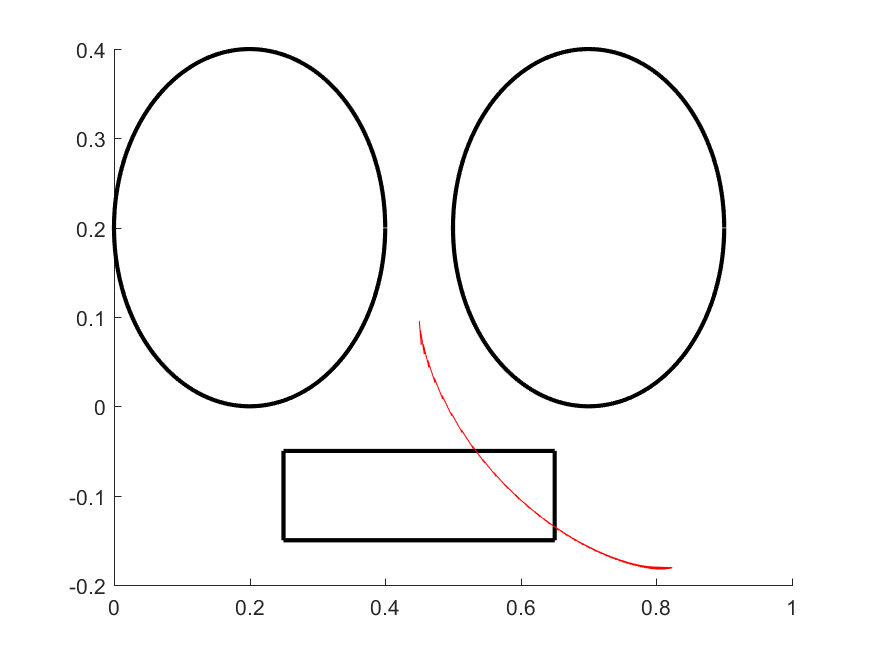
\includegraphics[width=1.2\textwidth]{demos/demo1}
		\caption{demo 1}
		\label{fig:demo 1}
	\end{subfigure}
	\hfill
	\begin{subfigure}[b]{0.40\textwidth}
		\centering
		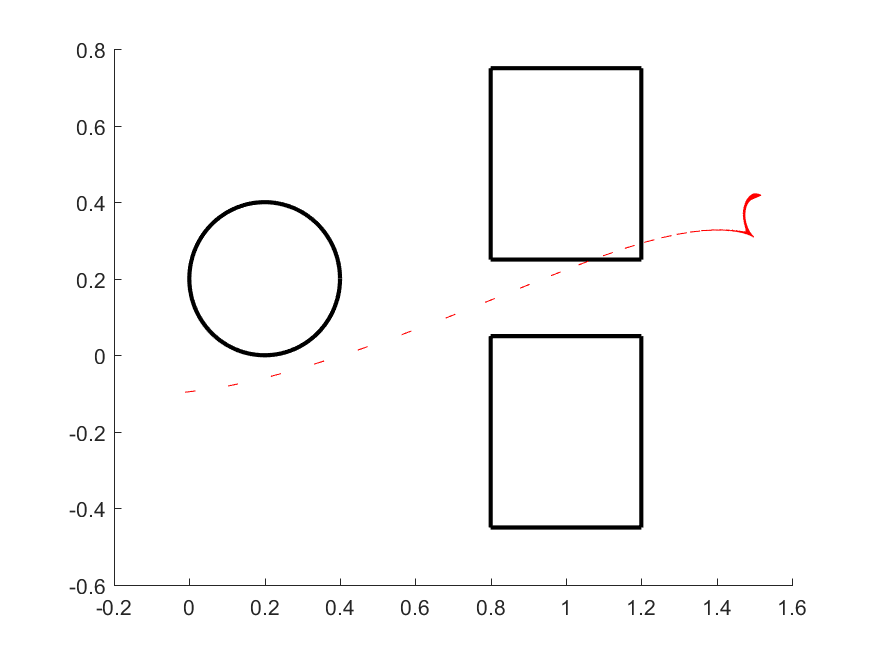
\includegraphics[width=1.2\textwidth]{demos/demo2}
		\caption{demo 2}
		\label{fig:demo 2}
	\end{subfigure}
	\begin{subfigure}[b]{0.40\textwidth}
		\centering
		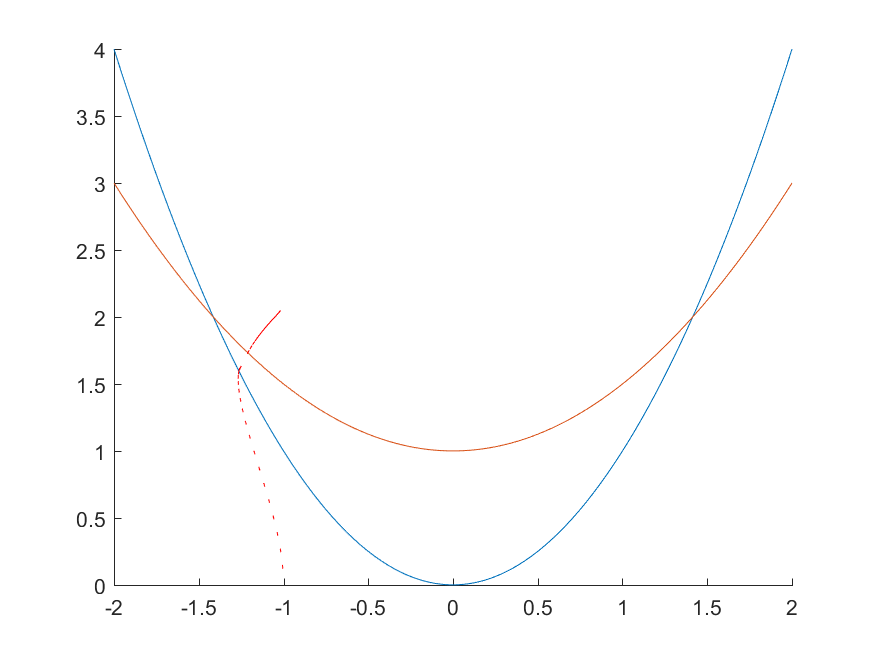
\includegraphics[width=1.2\textwidth]{demos/demo3}
		\caption{demo 3}
		\label{fig:demo 3}
	\end{subfigure}
	\hfill
	\begin{subfigure}[b]{0.40\textwidth}
		\centering
		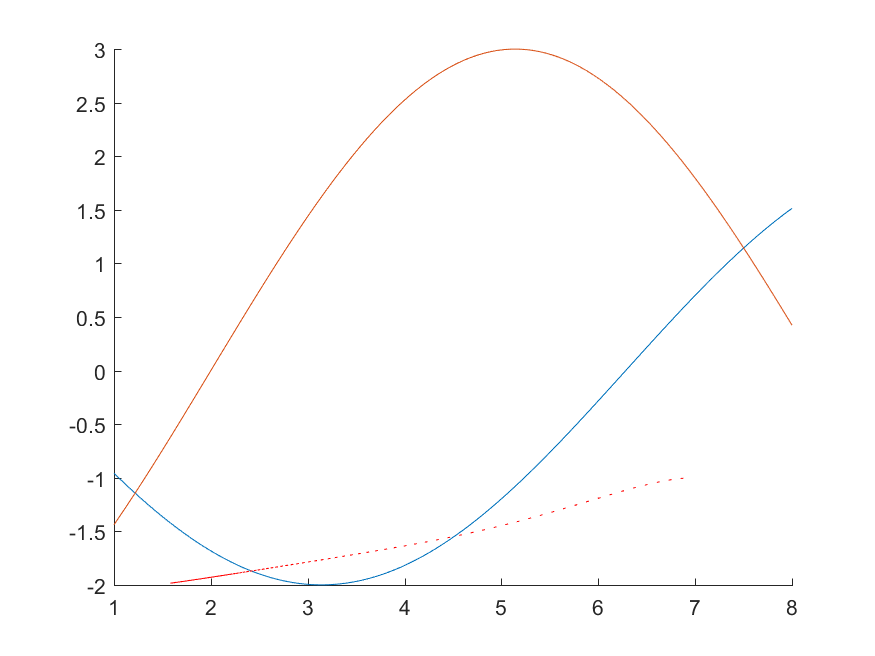
\includegraphics[width=1.2\textwidth]{demos/demo4}
		\caption{demo 4}
		\label{fig:demo 4}
	\end{subfigure}
	\caption{Path of demo's}
	\label{fig:demos}
\end{figure}
\begin{figure}[H]
	\centering
	\begin{subfigure}[b]{0.45\textwidth}
		\centering
		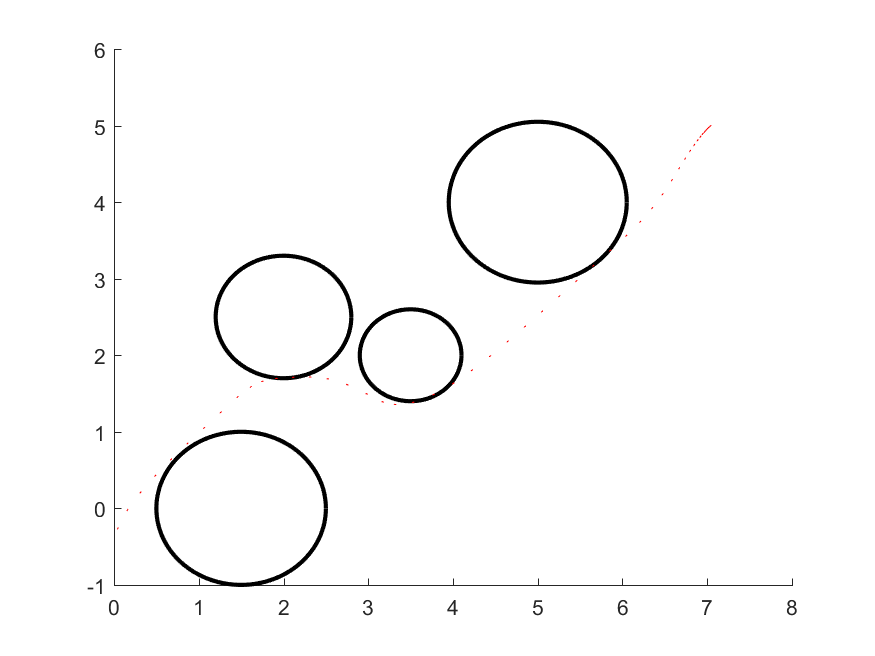
\includegraphics[width=1.2\textwidth]{demos/demo5}
		\caption{demo 5}
		\label{fig:demo 5}
	\end{subfigure}
\end{figure}

\section{Simulations without state noise}
\label{appendix:benchmarks trailer without noise}

\begin{table}[H]
	\centering
	\begin{tabular}{|l|c|c|c|c|}
		\hline
		&\textbf{demo5}&\textbf{demo2}&\textbf{demo3}\\\hline
		\textbf{nmpc-codegen}&9.00e-01&1.00e-01&4.10e-01\\\hline
		\textbf{PANOC Matab}&2.99e+01&4.20e+00&5.56e+00\\\hline
		\textbf{PANOC draft}&5.73e+00&1.29e+00&2.00e+00\\\hline
		\textbf{fmincon:interior-point}&8.62e+01&2.31e+01&2.03e+01\\\hline
		\textbf{fmincon:sqp}&2.18e+01&1.15e+01&9.29e+00\\\hline
		\textbf{fmincon:active-set}&8.37e+01&2.36e+01&2.08e+01\\\hline
		\textbf{OPTI:ipopt}&3.79e+01&7.08e+00&8.21e+00\\\hline
	\end{tabular}
	\caption{mean time till convergence in milliseconds}
	\label{tbl:mean time till convergence}
\end{table}

\begin{table}[H]
	\centering
	\begin{tabular}{|l|c|c|c|c|}
		\hline
		&\textbf{demo5}&\textbf{demo2}&\textbf{demo3}\\\hline
		\textbf{nmpc-codegen}&100&100&100\\\hline
		\textbf{PANOC Matab}&3323&4202&1357\\\hline
		\textbf{PANOC draft}&637&1289&489\\\hline
		\textbf{fmincon:interior-point}&9579&23107&4943\\\hline
		\textbf{fmincon:sqp}&2422&11469&2265\\\hline
		\textbf{fmincon:active-set}&9303&23578&5084\\\hline
		\textbf{OPTI:ipopt}&4213&7083&2003\\\hline
	\end{tabular}
	\caption{mean relative time till convergence in milliseconds}
	\label{tbl:mean relative time till convergence}
\end{table}

\begin{table}[H]
	\centering
	\begin{tabular}{|l|c|c|c|c|}
		\hline
		&\textbf{demo5}&\textbf{demo2}&\textbf{demo3}\\\hline
		\textbf{nmpc-codegen}&2.20e+01&8.00e+00&4.00e+01\\\hline
		\textbf{PANOC Matab}&7.95e+02&1.25e+02&3.06e+02\\\hline
		\textbf{PANOC draft}&1.12e+02&3.66e+01&1.30e+02\\\hline
		\textbf{fmincon:interior-point}&1.55e+03&2.29e+02&2.95e+02\\\hline
		\textbf{fmincon:sqp}&1.01e+02&8.83e+01&1.10e+02\\\hline
		\textbf{fmincon:active-set}&7.83e+02&2.70e+02&2.45e+02\\\hline
		\textbf{OPTI:ipopt}&2.73e+02&4.65e+01&7.65e+01\\\hline
	\end{tabular}
	\caption{max time till convergence in milliseconds}
	\label{tbl:max time till convergence}
\end{table}

\begin{table}[H]
	\centering
	\begin{tabular}{|l|	c|c|c|c|}
		\hline
		&\textbf{demo5}&\textbf{demo2}&\textbf{demo3}\\\hline
		\textbf{nmpc-codegen}&0.00e+00&0.00e+00&0.00e+00\\\hline
		\textbf{PANOC Matab}&2.11e+00&2.03e+00&2.01e+00\\\hline
		\textbf{PANOC draft}&5.16e-01&5.26e-01&5.16e-01\\\hline
		\textbf{fmincon:interior-point}&8.95e+00&8.35e+00&7.57e+00\\\hline
		\textbf{fmincon:sqp}&6.37e+00&6.58e+00&6.02e+00\\\hline
		\textbf{fmincon:active-set}&1.82e+01&1.63e+01&1.57e+01\\\hline
		\textbf{OPTI:ipopt}&5.03e+00&4.45e+00&4.37e+00\\\hline
	\end{tabular}
	\caption{min time till convergence in milliseconds}
	\label{tbl:min time till convergence}
\end{table}


\section{Simulations with state noise}
\label{appendix:benchmarks trailer with noise}

\begin{table}[H]
	\centering
	\begin{tabular}{|l|c|c|c|c|}
		\hline
		&\textbf{demo5}&\textbf{demo2}&\textbf{demo3}\\\hline
		\textbf{nmpc-codegen}&5.82e+00&4.20e-01&2.20e-01\\\hline
		\textbf{PANOC Matab}&8.69e+01&1.19e+01&9.64e+00\\\hline
		\textbf{PANOC draft}&2.77e+01&4.54e+00&3.24e+00\\\hline
		\textbf{fmincon:interior-point}&3.17e+02&1.01e+02&8.15e+01\\\hline
		\textbf{fmincon:sqp}&9.07e+01&4.77e+01&3.93e+01\\\hline
		\textbf{fmincon:active-set}&2.29e+02&7.50e+01&6.46e+01\\\hline
		\textbf{OPTI:ipopt}&9.52e+01&1.41e+01&1.09e+01\\\hline
	\end{tabular}
	\caption{mean time till convergence in milliseconds}
	\label{tbl:mean time till convergence with noise}
\end{table}

\begin{table}[H]
	\centering
	\begin{tabular}{|l|c|c|c|c|}
		\hline
		&\textbf{demo5}&\textbf{demo2}&\textbf{demo3}\\\hline
		\textbf{nmpc-codegen}&100&100&100\\\hline
		\textbf{PANOC Matab}&1494&2839&4383\\\hline
		\textbf{PANOC draft}&476&1080&1472\\\hline
		\textbf{fmincon:interior-point}&5453&24054&37058\\\hline
		\textbf{fmincon:sqp}&1560&11360&17870\\\hline
		\textbf{fmincon:active-set}&3937&17860&29378\\\hline
		\textbf{OPTI:ipopt}&1637&3362&4952\\\hline
	\end{tabular}
	\caption{mean relative time till convergence in milliseconds}
	\label{tbl:mean relative time till convergence with noise}
\end{table}

\begin{table}[H]
	\centering
	\begin{tabular}{|l|c|c|c|c|}
		\hline
		&\textbf{demo5}&\textbf{demo2}&\textbf{demo3}\\\hline
		\textbf{nmpc-codegen}&1.06e+02&1.30e+01&1.80e+01\\\hline
		\textbf{PANOC Matab}&9.82e+02&2.23e+02&3.87e+01\\\hline
		\textbf{PANOC draft}&2.38e+02&7.07e+01&1.83e+01\\\hline
		\textbf{fmincon:interior-point}&2.45e+03&4.68e+02&3.40e+02\\\hline
		\textbf{fmincon:sqp}&4.22e+02&3.25e+02&4.18e+02\\\hline
		\textbf{fmincon:active-set}&1.13e+03&4.86e+02&5.69e+02\\\hline
		\textbf{OPTI:ipopt}&4.78e+02&9.21e+01&3.67e+01\\\hline
	\end{tabular}
	\caption{max time till convergence in milliseconds}
	\label{tbl:max time till convergence with noise}
\end{table}

\begin{table}[H]
	\centering
	\begin{tabular}{|l|	c|c|c|c|}
		\hline
		&\textbf{demo5}&\textbf{demo2}&\textbf{demo3}\\\hline
		\textbf{nmpc-codegen}&0.00e+00&0.00e+00&0.00e+00\\\hline
		\textbf{PANOC Matab}&4.62e+00&3.55e+00&3.18e+00\\\hline
		\textbf{PANOC draft}&1.80e+00&1.26e+00&1.22e+00\\\hline
		\textbf{fmincon:interior-point}&4.85e+01&1.33e+01&1.05e+01\\\hline
		\textbf{fmincon:sqp}&1.44e+01&8.63e+00&9.95e+00\\\hline
		\textbf{fmincon:active-set}&3.48e+01&2.04e+01&1.72e+01\\\hline
		\textbf{OPTI:ipopt}&1.68e+01&4.67e+00&5.38e+00\\\hline
	\end{tabular}
	\caption{min time till convergence in milliseconds}
	\label{tbl:min time till convergence with noise}
\end{table}

\chapter{Poster}
\includepdf[pages={-},fitpaper,rotateoversize]{poster.pdf}